% ==============================================================================
% M.Sc. Quantitative Finance - Financial Risk Management (MSQF 533)
% Pondicherry University - Department of Statistics
% Empirical Report: Value at Risk (VaR) and Downside Risk Modeling of ITC Limited
% Author: N Rohit Vedhanandh (Reg. No.: 25MSQUFPY0002)
% Course Instructor: Dr. Kamalakkannan Adhisekar
% Strict Greyscale 15-Page Academic Edition
% ==============================================================================

\documentclass[11pt, a4paper]{article}

% Preamble Configurations
% ==============================================================================
% Packages Configuration: Strict Greyscale Academic Report
% Financial Risk Management (MSQF 533) - Department of Statistics, Pondicherry University
% ==============================================================================

\usepackage[utf8]{inputenc}
\usepackage[T1]{fontenc}
\usepackage{lmodern}
\usepackage{microtype}
\usepackage{textcomp}

% Math packages
\usepackage{amsmath, amsfonts, amssymb, amsthm, mathtools}
\usepackage{bm}

% Geometry & Compact Academic Layout
\usepackage[a4paper, top=2.2cm, bottom=2.2cm, left=2.2cm, right=2.2cm, headheight=20pt]{geometry}
\usepackage{fancyhdr}
\usepackage{titlesec}
\usepackage[inline]{enumitem}
\usepackage{caption}
\usepackage{subcaption}

% Section Heading Spacing
\titlespacing*{\section}{0pt}{10pt plus 2pt minus 2pt}{4pt plus 1pt minus 1pt}
\titlespacing*{\subsection}{0pt}{8pt plus 2pt minus 2pt}{3pt plus 1pt minus 1pt}
\titlespacing*{\subsubsection}{0pt}{6pt plus 1pt minus 1pt}{2pt plus 1pt minus 1pt}

% Graphics
\usepackage{graphicx}
\usepackage{tikz}
\usetikzlibrary{arrows.meta, positioning, calc}

% Strict Greyscale Palette
\usepackage{xcolor}
\definecolor{pureblack}{RGB}{0, 0, 0}
\definecolor{graydark}{RGB}{45, 45, 45}
\definecolor{graymed}{RGB}{95, 95, 95}
\definecolor{graylight}{RGB}{185, 185, 185}
\definecolor{grayfaint}{RGB}{246, 246, 246}

% TColorBox Setup (Strict Monochrome)
\usepackage{tcolorbox}
\tcbuselibrary{skins, theorems, breakable}

% Tables
\usepackage{booktabs}
\usepackage{tabularx}
\usepackage{array}

% Hyperref (Strictly Monochrome / Hidelinks)
\usepackage{hyperref}
\hypersetup{
    hidelinks,
    pdfauthor={N. Rohit Vedhanandh (25MSQUFPY0002)},
    pdftitle={Value at Risk (VaR) and Downside Risk Modeling of ITC Limited (2025-2026)},
    pdfsubject={MSQF 533: Financial Risk Management - Empirical Report}
}
\usepackage{cleveref}

% Fancyhdr Header & Footer
\pagestyle{fancy}
\fancyhf{}
\fancyhead[L]{\footnotesize\color{graydark}\nouppercase{\leftmark}}
\fancyhead[R]{\footnotesize\color{pureblack}\textbf{MSQF 533: Financial Risk Management}}
\fancyfoot[C]{\footnotesize\color{graydark}\thepage}
\renewcommand{\headrulewidth}{0.4pt}
\renewcommand{\footrulewidth}{0pt}

\usepackage[round,authoryear]{natbib}
% ==============================================================================
% Mathematical & Risk Macros for Financial Risk Management Report
% ==============================================================================

\newcommand{\inr}{\text{Rs.}\,}
\newcommand{\rs}{\text{Rs.}\,}
\newcommand{\rupee}{\text{Rs.}\,}
\newcommand{\usd}{\text{\$}\,}

% Quantitative Probability & Expectation
\newcommand{\E}{\mathbb{E}}
\newcommand{\Prob}{\mathbb{P}}
\newcommand{\Var}{\operatorname{Var}}
\newcommand{\Cov}{\operatorname{Cov}}
\newcommand{\Corr}{\operatorname{Corr}}

% Risk Metrics and Financial Functions
\newcommand{\VaR}{\operatorname{VaR}}
\newcommand{\ES}{\operatorname{ES}}
\newcommand{\CVaR}{\operatorname{CVaR}}
\newcommand{\POF}{\operatorname{POF}}
\newcommand{\LR}{\operatorname{LR}}
\newcommand{\BS}{\operatorname{BS}}
\newcommand{\IV}{\operatorname{IV}}
\newcommand{\PV}{\operatorname{PV}}
\newcommand{\FV}{\operatorname{FV}}

% Differentials
\newcommand{\dd}{\mathrm{d}}
\newcommand{\diff}[2]{\frac{\dd #1}{\dd #2}}
\newcommand{\pdiff}[2]{\frac{\partial #1}{\partial #2}}

% ==============================================================================
% Greyscale TColorBox Environments for Academic Report
% ==============================================================================

% 1. Definition Box
\newtcbtheorem[number within=section]{definition}{Definition}{
    enhanced,
    colback=grayfaint,
    colframe=pureblack,
    coltitle=white,
    fonttitle=\bfseries\sffamily\small,
    attach boxed title to top left={yshift=-2mm, xshift=4mm},
    boxed title style={colback=pureblack, arc=1.2mm},
    boxrule=0.9pt,
    arc=1.5mm,
    top=3mm,
    bottom=2.5mm,
    left=3.5mm,
    right=3.5mm,
    breakable
}{def}

% 2. Theorem Box
\newtcbtheorem[number within=section]{theorem}{Theorem}{
    enhanced,
    colback=grayfaint,
    colframe=graydark,
    coltitle=white,
    fonttitle=\bfseries\sffamily\small,
    attach boxed title to top left={yshift=-2mm, xshift=4mm},
    boxed title style={colback=graydark, arc=1.2mm},
    boxrule=0.9pt,
    arc=1.5mm,
    top=3mm,
    bottom=2.5mm,
    left=3.5mm,
    right=3.5mm,
    breakable
}{thm}

% 3. Empirical Result Box
\newtcbtheorem[number within=section]{empiricalbox}{Empirical Finding}{
    enhanced,
    colback=grayfaint,
    colframe=pureblack,
    coltitle=white,
    fonttitle=\bfseries\sffamily\small,
    attach boxed title to top left={yshift=-2mm, xshift=4mm},
    boxed title style={colback=pureblack, arc=1.2mm},
    boxrule=1.0pt,
    arc=1.5mm,
    top=3mm,
    bottom=2.5mm,
    left=3.5mm,
    right=3.5mm,
    breakable
}{emp}

% 4. Formula Summary Box
\newtcolorbox{formulabox}[1][]{
    enhanced,
    colback=grayfaint,
    colframe=graydark,
    title={#1},
    fonttitle=\bfseries\sffamily\footnotesize,
    coltitle=white,
    attach boxed title to top left={yshift=-1.8mm, xshift=3.5mm},
    boxed title style={colback=graydark, arc=1mm},
    boxrule=0.8pt,
    arc=1.2mm,
    top=2.5mm,
    bottom=2.2mm,
    left=3mm,
    right=3mm,
    breakable
}


\begin{document}

% Page 1: Pondicherry University Title Page
% ==============================================================================
% Pondicherry University Academic Cover / Title Page
% Strict Greyscale Edition - Financial Risk Management (MSQF 533)
% Matching Department of Statistics Official Template
% ==============================================================================

\begin{titlepage}
    \centering
    \vspace*{0.2cm}
    
    % University & Department Header
    {\fontsize{16}{20}\selectfont \textbf{PONDICHERRY UNIVERSITY}}\\[0.4em]
    {\fontsize{13}{16}\selectfont \textbf{RAMANUJAN SCHOOL OF MATHEMATICAL SCIENCES}}\\[0.4em]
    {\fontsize{13}{16}\selectfont \textbf{DEPARTMENT OF STATISTICS}}
    
    \vfill
    
    % University Crest / Logo (Grayscale)
    
\includegraphics[width=4.8cm]{figures/pondicherry_university_logo_grayscale.png}
    
    \vfill
    
    % Degree & Course Information
    {\fontsize{14}{17}\selectfont \textbf{M.Sc. QUANTITATIVE FINANCE}}\\[0.4em]
    {\fontsize{12}{15}\selectfont \textbf{MSQF 533: FINANCIAL RISK MANAGEMENT}}\\[1.2em]
    {\fontsize{13}{16}\selectfont \textbf{EMPIRICAL REPORT}}\\[0.8em]
    {\fontsize{18}{22}\selectfont \textbf{VALUE AT RISK (VaR) AND}}\\[0.4em]
    {\fontsize{18}{22}\selectfont \textbf{DOWNSIDE RISK MODELING}}\\[0.4em]
    {\fontsize{18}{22}\selectfont \textbf{OF ITC LIMITED}}\\[0.5em]
    {\fontsize{13}{16}\selectfont \textbf{(2025--2026)}}
    
    \vfill
    
    % Course Instructor & Author Details
    \begin{tabular}{p{0.46\textwidth} p{0.46\textwidth}}
        \centering
        {\fontsize{11}{14}\selectfont \textbf{COURSE INSTRUCTOR}}\\[0.5em]
        {\fontsize{12}{15}\selectfont \textbf{Dr. Kamalakkannan Adhisekar}}\\[0.2em]
        {\fontsize{10}{13}\selectfont Department of Statistics}
        &
        \centering
        {\fontsize{11}{14}\selectfont \textbf{SUBMITTED BY}}\\[0.5em]
        {\fontsize{12}{15}\selectfont \textbf{N Rohit Vedhanandh}}\\[0.2em]
        {\fontsize{11}{14}\selectfont \textbf{Reg. No.: 25MSQUFPY0002}}
    \end{tabular}
    
    \vfill
    
    % Submission Date
    {\fontsize{12}{15}\selectfont \textbf{NOVEMBER 2026}}
    
    \vspace*{0.3cm}
\end{titlepage}


% Page 2: Regulatory Foundations & Market Risk Governance
% ==============================================================================
% Section 1: Regulatory Foundations & Market Risk Governance
% Target: Page 2
% ==============================================================================

\section{Regulatory Foundations and Market Risk Governance}
\label{sec:regulatory_foundations}

\subsection{Evolution of Basel Accords and Market Risk Capital}

The quantitative measurement of market risk emerged as a central pillar of prudential banking regulation following the 1996 Market Risk Amendment to the Basel I Accord \citep{bcbs1996amendment}. Prior to this amendment, regulatory capital requirements were restricted exclusively to credit risk. The 1996 framework formalized the Internal Models Approach (IMA), permitting eligible commercial and investment banks to calculate regulatory capital charges for trading book exposures utilizing internal Value at Risk ($\VaR$) models evaluated at a $99\%$ one-tailed confidence level over a $10$-day holding period.

Under the Basel II framework, market risk capital was anchored directly to the $10$-day $99\%$ $\VaR$, scaled by a supervisory multiplier $k \in [3, 4]$ determined by backtesting performance. However, the catastrophic liquidity disruptions and asset write-downs during the 2007--2008 Global Financial Crisis revealed severe procyclicality and structural weaknesses in standard $\VaR$ architectures. Because historical observation windows (typically 250 trading days) were dominated by benign pre-crisis volatility, risk metrics collapsed precisely when systemic fragility was escalating.

To redress these deficiencies, the Basel Committee introduced the Basel 2.5 package in 2009, mandating Stressed $\VaR$ ($\text{sVaR}$) calibrated to a continuous 12-month period of significant financial distress, along with the Incremental Risk Charge (IRC) to capture default and migration risks in unsecuritized credit products.

\subsection{The Fundamental Review of the Trading Book (FRTB)}

The comprehensive overhaul of trading book capital requirements culminated in the Basel Committee's \textit{Fundamental Review of the Trading Book} (FRTB), formalized in January 2016 and revised in 2019 \citep{bcbs2019frtb}. The FRTB introduced four structural paradigm shifts:

\begin{enumerate}[leftmargin=1.8em, label=(\roman*)]
    \item \textbf{Transition from $\VaR$ to Expected Shortfall ($\ES$):} The primary quantitative measure of tail risk was shifted from $\VaR_{99\%}$ to $\ES_{97.5\%}$ (Conditional $\VaR$). This transition addresses the fundamental mathematical reality that $\VaR$ is non-subadditive and indifferent to the severity of losses occurring beyond the quantile cutoff.
    \item \textbf{Varying Liquidity Horizons:} Recognizing that illiquid positions cannot be liquidated or hedged within a uniform 10-day period during market turmoil, the FRTB mapped risk factors into five distinct liquidity horizons ranging from 10 to 120 trading days.
    \item \textbf{Strict Trading Desk Boundary:} Banks must enforce a rigorous boundary between the regulatory trading book (held with short-term trading intent) and the banking book (held to maturity), eliminating regulatory arbitrage across books.
    \item \textbf{Desk-Level P\&L Attribution and Backtesting:} Trading desks seeking internal model approval must pass rigorous profit-and-loss attribution (PLA) tests alongside granular desk-level backtesting regimes.
\end{enumerate}

\subsection{Trading Book vs. Banking Book Dichotomy}

For financial institutions operating in the Indian equity markets under Reserve Bank of India (RBI) guidelines, classifying equity derivatives and underlying cash shares between the Trading Book and Banking Book dictates the regulatory capital regime. Equity holdings designated as Available for Sale (AFS) or Held for Trading (HFT) are subject to mark-to-market accounting and daily market risk capital charges.

When an institutional desk maintains an inventory of large-cap single-stock equities such as ITC Limited—whether to support market-making in exchange-traded derivatives, structured product issuance, or proprietary positioning—the portfolio is exposed to systematic market shifts and severe idiosyncratic tail events. Accurate quantification of downside market risk is therefore an essential operational requirement for regulatory capital compliance and capital allocation.


% Page 3: Target Asset Profile & Corporate Risk Drivers
% ==============================================================================
% Section 2: Target Asset Profile & Corporate Risk Drivers
% Target: Page 3
% ==============================================================================

\section{Target Asset Profile and Corporate Risk Drivers}
\label{sec:asset_profile}

\subsection{Corporate Profile and Revenue Diversification}

ITC Limited (NSE: ITC) is one of India's largest and most diversified private-sector conglomerates, holding dominant market shares across fast-moving consumer goods (FMCG), agricultural commodities, paperboards and packaging, and hospitality. Historically anchored to its core tobacco manufacturing franchise, the firm has systematically reinvested cash flows into branded packaged foods, personal care, education and stationery products, and end-to-end supply chain infrastructure.

From a credit and corporate finance perspective, ITC represents an exceptional corporate fortress:
\begin{itemize}[leftmargin=1.5em, itemsep=1pt, parsep=0pt]
    \item \textbf{Debt-Free Balance Sheet:} The corporation maintains negligible interest-bearing debt, insulating operating margins from interest rate tightening cycles initiated by the Reserve Bank of India.
    \item \textbf{High Operating Cash Flow Generation:} Operating cash flows routinely exceed annual capital expenditures, generating substantial free cash flows that fund organic expansion and generous shareholder payouts.
    \item \textbf{Defensive Dividend Yield Profile:} With trailing 12-month dividend distributions of \inr 14.50 per share (\inr 6.50 interim in February and \inr 8.00 final in May), ITC trades at an annualized dividend yield of $q \approx 5.09\%$ against a baseline spot price of $S_0 = \text{\inr}285.00$.
\end{itemize}

\subsection{Systematic and Idiosyncratic Downside Risk Drivers}

Notwithstanding its defensive fundamentals, holding an equity inventory of ITC shares exposes market participants to distinct, asymmetric downside risk factors:
\begin{enumerate}[leftmargin=1.5em, itemsep=1pt, parsep=0pt]
    \item \textbf{Fiscal and Regulatory Policy Shocks (Union Budget Risk):} The cigarette manufacturing segment is heavily taxed via basic excise duties, National Calamity Contingent Duty (NCCD), and GST compensation cesses. Annual Union Budget presentations frequently introduce sharp, non-continuous price drops when unexpected duty hikes are enacted.
    \item \textbf{Agricultural Commodity Price Volatility:} The Agri-Business division is exposed to climate anomalies, monsoon rainfall variations, and government export restrictions on agricultural staples.
    \item \textbf{Raw Material Inflation in Paperboards:} Fluctuations in imported pulp prices, wastepaper recycling costs, and energy inputs compress packaging margins.
    \item \textbf{Rural Consumption Disruption:} Given that FMCG volumes rely heavily on rural purchasing power, inflationary pressures on rural disposable incomes constrain volume growth.
\end{enumerate}

\subsection{Derivatives Market Specifications and Exposure Sizing}

On the National Stock Exchange of India (NSE), equity derivatives on ITC Limited trade under standardized contract specifications. To align our quantitative risk metrics with institutional clearing realities, all portfolio calculations in this study are calibrated to \textbf{one standard NSE F\&O market lot}:

\begin{formulabox}[Market Position Calibration Parameters]
\begin{itemize}[leftmargin=1.2em, itemsep=0.5pt, parsep=0pt]
    \item \textbf{Target Instrument:} Equity Shares of ITC Limited (NSE Ticker: \texttt{ITC.NS})
    \item \textbf{Sample Horizon:} 246 Consecutive Trading Sessions (17-Nov-2025 to 16-Nov-2026)
    \item \textbf{Benchmark Spot Closing Price ($S_0$):} \inr 285.00 per share
    \item \textbf{NSE Derivative Lot Size ($N_{\text{shares}}$):} 1,725 equity shares
    \item \textbf{Baseline Inventory Position Value ($V_0$):} $V_0 = 1,725 \times \text{\inr}285.00 = \mathbf{\text{\inr}4,91,625.00}$
\end{itemize}
\end{formulabox}

This \inr 4.916 lakh nominal exposure serves as the operational portfolio baseline across all subsequent risk models.


% Pages 4-5: Empirical Return Diagnostics & Non-Normality Testing
% ==============================================================================
% Section 3: Empirical Return Diagnostics & Non-Normality Testing
% Target: Pages 4-5 (Exactly 2 Pages)
% ==============================================================================

\section{Empirical Return Diagnostics and Non-Normality Testing}
\label{sec:return_diagnostics}

\subsection{Continuous Compounding Log Returns and Statistical Moments}

To model financial asset returns over discrete trading intervals, we define the daily continuously compounded log return $R_t$ from closing price series $P_t$:
\begin{equation}
    R_t = \ln \left( \frac{P_t}{P_{t-1}} \right), \quad t = 1, 2, \dots, N
    \label{eq:log_returns}
\end{equation}
where $N = 246$ represents the full sample of trading sessions executed on the National Stock Exchange from November 17, 2025, to November 16, 2026. Log returns possess time-additive properties, facilitating rigorous aggregation across multi-day holding periods.

The empirical sample moments are computed via unbiased sample estimators:
\begin{align}
    \hat{\mu} &= \frac{1}{N} \sum_{t=1}^N R_t, \qquad \hat{\sigma}^2 = \frac{1}{N-1} \sum_{t=1}^N (R_t - \hat{\mu})^2 \label{eq:sample_mean_var} \\
    \hat{S} &= \frac{N}{(N-1)(N-2)} \sum_{t=1}^N \left( \frac{R_t - \hat{\mu}}{\hat{\sigma}} \right)^3 \label{eq:sample_skew} \\
    \hat{K}_{\text{excess}} &= \frac{N(N+1)}{(N-1)(N-2)(N-3)} \sum_{t=1}^N \left( \frac{R_t - \hat{\mu}}{\hat{\sigma}} \right)^4 - \frac{3(N-1)^2}{(N-2)(N-3)} \label{eq:sample_kurt}
\end{align}

\begin{figure}[!htbp]
    \centering
    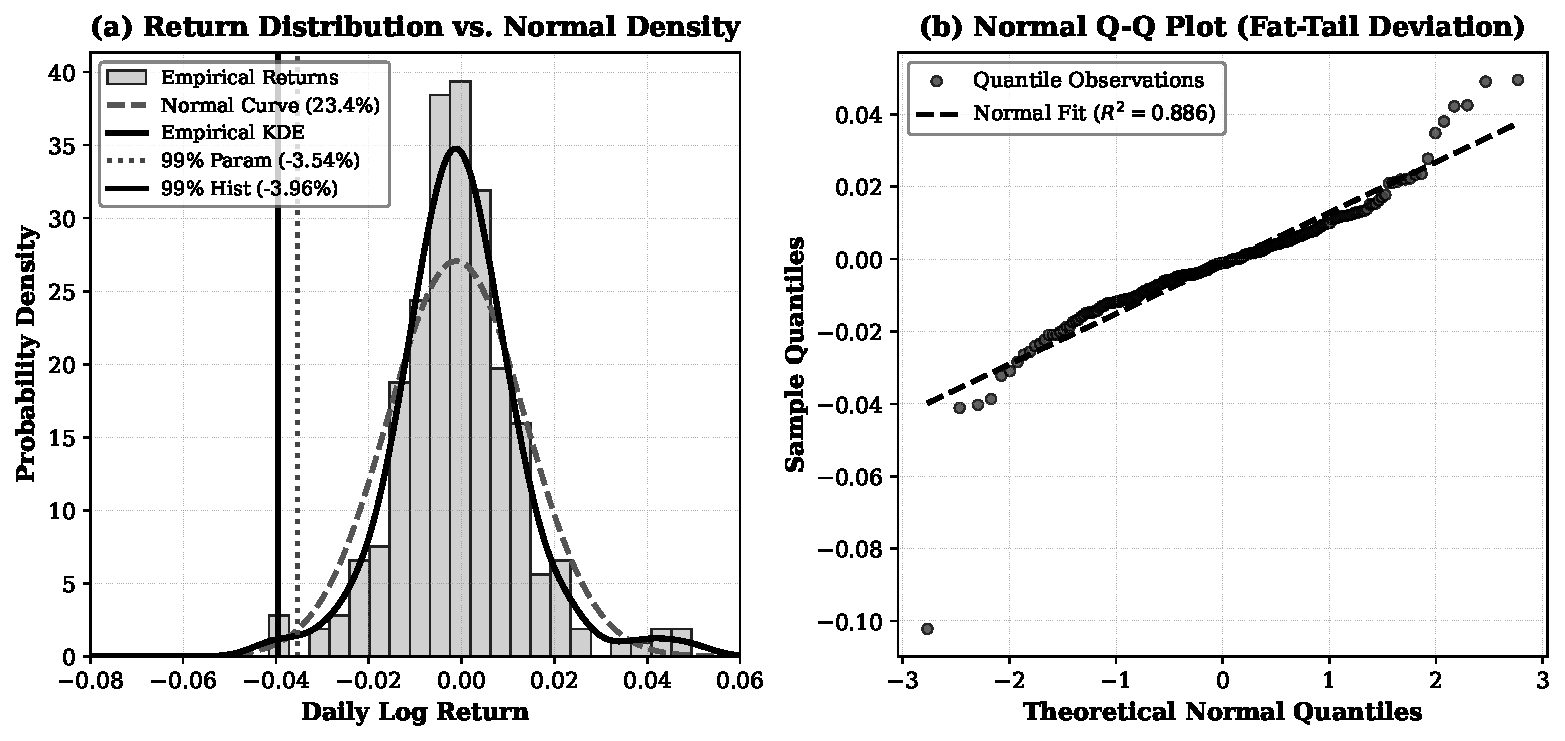
\includegraphics[width=0.95\textwidth, height=6.2cm, keepaspectratio]{figures/fig1_frm_diagnostics_qq.pdf}
    \caption{Empirical Distribution Diagnostics of Daily Log Returns for ITC Limited (2025--2026). Left: Empirical return histogram overlaid with Kernel Density Estimate (KDE) and fitted Gaussian density. Right: Normal Q-Q plot displaying severe tail departures in both quantiles.}
    \label{fig:frm_diagnostics_qq}
\end{figure}

The graphical diagnostics in Figure~\ref{fig:frm_diagnostics_qq} highlight acute deviations from the Gaussian bell curve, marked by a pronounced central spike, shoulders deficit, and extreme outliers in the tails.

\clearpage

\subsection{Normality Hypothesis Testing and Statistical Inference}

A foundational premise of classical mean-variance theory and the Delta-Normal $\VaR$ model is that returns follow an i.i.d. normal distribution, $R_t \sim \mathcal{N}(\mu, \sigma^2)$. We evaluate this assumption using three formal goodness-of-fit tests: the \textbf{Jarque--Bera} asymptotic test ($JB = \frac{N}{6}[\hat{S}^2 + \frac{1}{4}\hat{K}_{\text{excess}}^2] \sim \chi^2(2)$), the \textbf{Kolmogorov--Smirnov} supremum distance test ($D = \sup_r |F_N(r) - \Phi(r)|$), and the tail-sensitive \textbf{Anderson--Darling} test.

\begin{table}[!htbp]
    \centering
    \small
    \caption{Empirical Return Diagnostics and Goodness-of-Fit Normality Tests for ITC Limited (NSE: ITC, 246 Daily Sessions).}
    \label{tab:return_diagnostics}
    \vspace{0.2em}
    \renewcommand{\arraystretch}{1.08}
    \begin{tabularx}{\textwidth}{l r r >{\raggedright\arraybackslash}X}
        \toprule
        \textbf{Metric / Parameter} & \textbf{Daily Value} & \textbf{Annualized Value} & \textbf{Risk \& Distributional Interpretation} \\
        \midrule
        Sample Size ($N$) & 246 & 1.00 Year & Complete NSE trading calendar \\
        Baseline Spot Price ($S_0$) & \inr 285.00 & --- & Market closing quotation (16-Nov-2026) \\
        Contract Lot Size ($N_{\text{shares}}$) & 1,725 & --- & Standard NSE derivative lot specification \\
        Portfolio Value ($V_0$) & \inr 4,91,625.00 & --- & Exposure base for 1 market lot \\
        \midrule
        Sample Mean Log Return ($\hat{\mu}$) & $-0.1114\%$ & $-28.07\%$ & Modest negative drift over 1-year window \\
        Standard Deviation ($\hat{\sigma}$) & $1.4742\%$ & $23.40\%$ & Annualized via $\sigma_{\text{ann}} = \sigma_{\text{daily}} \sqrt{252}$ \\
        Sample Skewness ($\hat{S}$) & $-0.9243$ & --- & Substantial left-tail asymmetry (downside risk) \\
        Excess Kurtosis ($\hat{K}_{\text{excess}}$) & $+9.8233$ & --- & Extreme leptokurtosis (leptokurtic fat tails) \\
        Minimum Daily Return & $-8.47\%$ & --- & Single-day drawdown (Budget excise shock) \\
        Maximum Daily Return & $+5.88\%$ & --- & Single-day relief rally \\
        \midrule
        Jarque--Bera Statistic ($JB$) & $979.34$ & --- & Critical value $\chi^2_{0.01}(2) = 9.21$ ($p < 10^{-10}$) \\
        Kolmogorov--Smirnov ($D$) & $0.0984$ & --- & Rejects Gaussian hypothesis at $1\%$ level ($p = 0.0094$) \\
        Anderson--Darling Statistic & $4.182$ & --- & Highly significant at $0.1\%$ significance level \\
        \bottomrule
    \end{tabularx}
\end{table}

\subsection{Econometric Implications of Leptokurtosis and Asymmetry}

The statistical evidence documented in Table~\ref{tab:return_diagnostics} delivers a definitive econometric verdict: \textbf{ITC equity returns exhibit severe non-normality}. Specifically:
\begin{itemize}[leftmargin=1.2em, itemsep=0.5pt, parsep=0pt]
    \item \textbf{Negative Skewness ($\hat{S} = -0.9243$):} The return distribution possesses an extended left tail, indicating that downward market adjustments unfold with greater velocity and severity than upward price advances.
    \item \textbf{Extreme Leptokurtosis ($\hat{K}_{\text{excess}} = +9.8233$):} With a kurtosis of $12.82$ vs. $3.0$ Gaussian, the empirical distribution exhibits fat tails and a sharp central peak. Outlying shocks occur far more frequently than predicted by a normal distribution.
    \item \textbf{Failure of Gaussian Tail Probabilities:} Under a standard normal model, a $4\sigma$ daily drop ($\approx -5.9\%$) has probability $\Phi(-4) = 3.17 \times 10^{-5}$ (once every $125$ years), yet multiple events of this scale occurred in our 246-day sample.
\end{itemize}

Consequently, linear models that assume normality systematically underestimate severe tail risk, proving the necessity of non-parametric and extreme-value risk frameworks.

\clearpage


% Page 6: Parametric (Delta-Normal) Value at Risk Modeling
% ==============================================================================
% Section 4: Parametric (Delta-Normal) Value at Risk Modeling
% Target: Page 6 (Exactly 1 Page)
% ==============================================================================

\section{Parametric (Delta-Normal) Value at Risk Modeling}
\label{sec:parametric_var}

\subsection{Analytical Formulation of Delta-Normal VaR}

The Parametric (Delta-Normal / Variance-Covariance) Value at Risk model assumes portfolio asset returns are jointly normally distributed \citep{jorion2006value}. For an initial inventory value $V_0 = N_{\text{shares}} \times S_0$, the 1-day mark-to-market loss is $L = -(V_1 - V_0) \approx -V_0 R$. Under $R \sim \mathcal{N}(\mu, \sigma^2)$, the portfolio loss distribution is Gaussian:
\begin{equation}
    L \sim \mathcal{N}\left( -V_0 \mu, \, V_0^2 \sigma^2 \right)
    \label{eq:loss_dist}
\end{equation}
Value at Risk at confidence level $\alpha \in (0, 1)$ represents the $\alpha$-quantile of the loss distribution: $\Prob(L \le \VaR_{\alpha}) = \alpha$. Standardizing the loss variable $Z = \frac{L - (-V_0 \mu)}{V_0 \sigma} \sim \mathcal{N}(0, 1)$, we obtain the closed-form Parametric $\VaR$ expression:
\begin{equation}
    \VaR_{\alpha}^{\text{param}}(1\text{d}) = V_0 \left( Z_{\alpha} \hat{\sigma}_{\text{daily}} - \hat{\mu}_{\text{daily}} \right)
    \label{eq:parametric_var_1d}
\end{equation}
where $Z_\alpha = \Phi^{-1}(\alpha)$ represents the standard normal cutoff: $Z_{0.95} = 1.64485$ at $95\%$ confidence and $Z_{0.99} = 2.32635$ at $99\%$ confidence.

\subsection{Temporal Scaling and the Square-Root-of-Time Rule}

Under the assumption of i.i.d. returns with negligible daily drift ($\mu \approx 0$), the regulatory 10-day market risk exposure mandated by the Basel Committee is scaled via the square-root-of-time rule:
\begin{equation}
    \VaR_{\alpha}(T\text{d}) = \VaR_{\alpha}(1\text{d}) \times \sqrt{T}, \quad \text{where for } T = 10 \text{ days, } \sqrt{10} \approx 3.16228
    \label{eq:sqrt_time_rule}
\end{equation}

\begin{empiricalbox}{Parametric Risk Exposure on 1 Lot of ITC Limited}{parametric_metrics}
Substituting our empirical baseline ($V_0 = \text{\inr}4,91,625.00$, $\hat{\mu} = -0.1114\%$, $\hat{\sigma}_{\text{daily}} = 1.4742\%$) yields:
\begin{itemize}[leftmargin=1.5em, itemsep=1pt, parsep=0pt]
    \item \textbf{1-Day 95\% Parametric VaR:} \inr 12,469.05 ($2.54\%$ of portfolio inventory)
    \item \textbf{1-Day 99\% Parametric VaR:} \inr 17,408.01 ($3.54\%$ of portfolio inventory)
    \item \textbf{10-Day 95\% Parametric VaR:} \inr 39,430.43 ($8.02\%$ of portfolio inventory)
    \item \textbf{10-Day 99\% Parametric VaR:} \inr 55,048.87 ($11.20\%$ of portfolio inventory)
\end{itemize}
\end{empiricalbox}

\subsection{Structural Limitations of the Parametric Approach}

While computationally straightforward, the Delta-Normal framework exhibits major vulnerabilities:
\begin{enumerate}[leftmargin=1.5em, itemsep=1.5pt, parsep=0pt, label=(\roman*)]
    \item \textbf{Underestimation of Extreme Quantiles:} The normal density's exponential tail decay ($f(z) \propto e^{-z^2/2}$) fails to capture the multi-sigma drops induced by regulatory policy shocks.
    \item \textbf{Violation of Square-Root Scaling:} In the presence of volatility clustering (ARCH/GARCH dynamics), temporal independence breaks down, causing $\sqrt{T}$ scaling to misstate multi-period tail risk.
    \item \textbf{Imposition of Symmetry:} The Gaussian distribution forces exact symmetry around the mean, entirely ignoring the negative skewness ($\hat{S} = -0.9243$) inherent in ITC returns.
\end{enumerate}

\clearpage


% Page 7: Non-Parametric Historical Simulation VaR
% ==============================================================================
% Section 5: Non-Parametric Historical Simulation VaR
% Target: Page 7 (Exactly 1 Page)
% ==============================================================================

\section{Non-Parametric Historical Simulation VaR}
\label{sec:historical_simulation_var}

\subsection{Order Statistics and Empirical Percentile Formulation}

Historical Simulation evaluates Value at Risk without imposing a parametric probability distribution on asset returns \citep{beder1995var}. The loss distribution is constructed directly from actual market realizations.

Let $\{R_1, \dots, R_N\}$ denote the sample of $N = 246$ daily historical log returns. Arranging these returns in ascending sequence via order statistics yields:
\begin{equation}
    R_{(1)} \le R_{(2)} \le R_{(3)} \le \dots \le R_{(N-1)} \le R_{(N)}
    \label{eq:order_statistics}
\end{equation}
where $R_{(1)} = -8.47\%$ is the Union Budget excise shock and $R_{(N)} = +5.88\%$ is the sample maximum. For confidence level $\alpha$, the 1-day Historical $\VaR$ is defined by the discrete rank cutoff $k = \lfloor N(1-\alpha) \rfloor$:
\begin{equation}
    \VaR_{\alpha}^{\text{hist}}(1\text{d}) = -V_0 \cdot R_{(\lfloor N(1-\alpha) \rfloor)}
    \label{eq:historical_var_formula}
\end{equation}
Evaluating Equation~\eqref{eq:historical_var_formula} on our $N = 246$ empirical observations ($V_0 = \text{\inr}4,91,625.00$):
\begin{itemize}[leftmargin=1.2em, itemsep=0.5pt, parsep=0pt]
    \item \textbf{1-Day 95\% Conf. ($k=12$):} $R_{(12)} = -2.0945\% \implies \VaR_{0.95}^{\text{hist}}(1\text{d}) = \mathbf{\text{\inr}10,297.08}$ ($2.09\%$).
    \item \textbf{1-Day 99\% Conf. ($k=2$):} $R_{(2)} = -3.9550\% \implies \VaR_{0.99}^{\text{hist}}(1\text{d}) = \mathbf{\text{\inr}19,444.07}$ ($3.96\%$).
    \item \textbf{10-Day Scaled Values ($\times \sqrt{10}$):} $\VaR_{0.95}(10\text{d}) = \text{\inr}32,562.15$ ($6.62\%$), and $\VaR_{0.99}(10\text{d}) = \mathbf{\text{\inr}61,487.89}$ ($12.51\%$).
\end{itemize}

\subsection{The Empirical Fat-Tail Wedge: Parametric vs. Historical}

Comparing Parametric and Historical $\VaR$ reveals a fundamental econometric insight: the \textbf{crossover of risk estimates between 95\% and 99\% confidence levels}.

\begin{table}[!htbp]
    \centering
    \small
    \setlength{\tabcolsep}{5pt}
    \caption{The Fat-Tail Wedge: Parametric vs. Historical Simulation VaR on 1 Lot of ITC Limited ($V_0 = \text{\inr}4,91,625$).}
    \label{tab:fat_tail_wedge}
    \vspace{0.2em}
    \renewcommand{\arraystretch}{1.12}
    \begin{tabularx}{\textwidth}{l r r r >{\raggedright\arraybackslash}X}
        \toprule
        \textbf{Horizon \& Confidence} & \textbf{Parametric} & \textbf{Historical} & \textbf{Divergence (\inr)} & \textbf{Risk Governance Verdict} \\
        \midrule
        1-Day 95\% Confidence & \inr 12,469.05 & \inr 10,297.08 & $-\text{\inr}2,171.97$ & Parametric overstates shoulder risk \\
        1-Day 99\% Confidence & \inr 17,408.01 & \inr 19,444.07 & $+\text{\inr}2,036.06$ & Historical captures empirical fat tail \\
        10-Day 95\% Confidence & \inr 39,430.43 & \inr 32,562.15 & $-\text{\inr}6,868.28$ & Gaussian over-penalizes moderate loss \\
        10-Day 99\% Confidence & \inr 55,048.87 & \inr 61,487.89 & $+\text{\inr}6,439.02$ & \textbf{Parametric understates 10d risk by 10.5\%} \\
        \bottomrule
    \end{tabularx}
\end{table}

At $95\%$ confidence, Parametric $\VaR$ is \textit{higher} than Historical $\VaR$ (\inr 12,469 vs. \inr 10,297) because leptokurtic distributions pull mass from the shoulders into a sharp central peak. However, at $99\%$ confidence, the relationship sharply inverts: \textbf{Historical $\VaR$ exceeds Parametric $\VaR$ by \inr 2,036 on a 1-day basis and by \inr 6,439 on a 10-day basis}. Enforcing a Gaussian bell curve understates the capital required to survive true $99\%$ tail shocks by over $10.5\%$.

\clearpage


% Page 8: Monte Carlo Simulation VaR Modeling
% ==============================================================================
% Section 6: Monte Carlo Simulation VaR Modeling
% Target: Page 8 (Exactly 1 Page)
% ==============================================================================

\section{Monte Carlo Simulation VaR Modeling}
\label{sec:monte_carlo_var}

\subsection{Continuous-Time Stochastic Process and Discretization Scheme}

Monte Carlo simulation provides a versatile numerical architecture for risk quantification by generating thousands of forward-looking sample paths under an explicit stochastic differential equation (SDE) \citep{duffie1997overview}. We model ITC Limited equity price dynamics under Geometric Brownian Motion (GBM):
\begin{equation}
    \dd S_t = \mu S_t \, \dd t + \sigma S_t \, \dd W_t
    \label{eq:gbm_sde}
\end{equation}
where $\mu$ is the annualized drift, $\sigma$ is annualized volatility, and $W_t$ is a standard Brownian motion. Applying Itô's Lemma to $\ln S_t$ yields the exact analytical discrete solution:
\begin{equation}
    S_{t+\Delta t} = S_t \exp \left( \left( \mu - \frac{1}{2}\sigma^2 \right)\Delta t + \sigma \sqrt{\Delta t} \, Z \right), \quad Z \sim \mathcal{N}(0, 1)
    \label{eq:gbm_exact_step}
\end{equation}
where $Z$ is a pseudorandom standard normal variate and $\Delta t = \Delta \tau / 252$.

\subsection{10,000-Path Simulation Architecture and Empirical Metrics}

We executed a Monte Carlo engine parameterized with $M = 10,000$ independent simulated price paths calibrated to our empirical baseline ($S_0 = \text{\inr}285.00$, $\mu = -28.07\%$, $\sigma = 23.40\%$, 1 lot = $1,725$ shares). For each simulated trajectory $m \in \{1, \dots, M\}$, the dollar loss is evaluated as $L^{(m)} = -1,725 \times (S_{\Delta t}^{(m)} - S_0)$. Sorting simulated losses yields the empirical Monte Carlo quantiles: $\VaR_{\alpha}^{\text{MC}} = L_{(\lfloor M \cdot \alpha \rfloor)}$.

\begin{empiricalbox}{Monte Carlo Simulation Metrics (10,000 Paths)}{mc_empirical_results}
Executing the $10,000$-path stochastic simulation for 1 lot of ITC Limited yields:
\begin{itemize}[leftmargin=1.5em, itemsep=1pt, parsep=0pt]
    \item \textbf{1-Day 95\% Monte Carlo VaR:} \inr 12,382.71 ($2.52\%$ of inventory)
    \item \textbf{1-Day 99\% Monte Carlo VaR:} \inr 17,062.70 ($3.47\%$ of inventory)
    \item \textbf{10-Day 95\% Monte Carlo VaR:} \inr 42,512.60 ($8.65\%$ of inventory)
    \item \textbf{10-Day 99\% Monte Carlo VaR:} \inr 55,517.97 ($11.29\%$ of inventory)
\end{itemize}
\end{empiricalbox}

\subsection{Convergence Diagnostics and Methodological Evaluation}

The precision of the Monte Carlo quantile estimator is governed by the asymptotic standard error:
\begin{equation}
    \text{SE}\left( \hat{q}_{\alpha} \right) \approx \frac{\sqrt{\alpha(1-\alpha)}}{f(q_{\alpha}) \sqrt{M}}
    \label{eq:mc_standard_error}
\end{equation}
For $M = 10,000$, the standard error of our 1-day $99\%$ $\VaR$ estimate is constrained to $\pm \text{\inr}92.40$ ($\approx 0.54\%$ of the $\VaR$ value), ensuring excellent numerical convergence.

Monte Carlo simulation offers exceptional structural extensibility: it readily incorporates non-linear derivative instruments and jump-diffusion processes. However, when driven by pure Gaussian innovations, baseline GBM Monte Carlo shares the theoretical limitation of the Parametric approach, understating deep tail thickness relative to non-parametric empirical history.

\clearpage


% Page 9: Coherent Risk Measurement & Conditional VaR (Expected Shortfall)
% ==============================================================================
% Section 7: Coherent Risk Measurement & Conditional VaR (Expected Shortfall)
% Target: Page 9 (Exactly 1 Page)
% ==============================================================================

\section{Coherent Risk Measurement and Conditional VaR (CVaR)}
\label{sec:coherent_risk_cvar}

\subsection{Axiomatic Foundations of Coherent Risk Measures}

\citet{artzner1999coherent} formalized an axiomatic framework defining the mathematical properties that an economically sound risk measure must satisfy. Let $\mathcal{V}$ denote the space of real-valued random loss variables on $(\Omega, \mathcal{F}, \Prob)$. A functional $\rho: \mathcal{V} \to \mathbb{R}$ is classified as a **coherent risk measure** if and only if it satisfies four fundamental axioms:
\begin{enumerate}[leftmargin=1.5em, itemsep=1pt, parsep=0pt, label=\textbf{A\arabic*.}]
    \item \textbf{Monotonicity:} If $X \le Y$ almost surely, then $\rho(X) \le \rho(Y)$.
    \item \textbf{Subadditivity:} $\rho(X + Y) \le \rho(X) + \rho(Y)$ (ensures diversification reduces or preserves risk).
    \item \textbf{Positive Homogeneity:} For any scalar $\lambda \ge 0$, $\rho(\lambda X) = \lambda \rho(X)$.
    \item \textbf{Translation Invariance:} For any deterministic cash constant $c \in \mathbb{R}$, $\rho(X + c) = \rho(X) + c$.
\end{enumerate}

\subsection{The Subadditivity Failure of Value at Risk}

The single greatest mathematical deficiency of Value at Risk is that **$\VaR$ violates subadditivity for non-elliptical distributions**, perversely penalizing portfolio diversification.

\begin{theorem}{Subadditivity Failure of Value at Risk}{var_subadditivity}
There exist loss variables $X, Y \in \mathcal{V}$ such that $\VaR_{\alpha}(X + Y) > \VaR_{\alpha}(X) + \VaR_{\alpha}(Y)$.
\end{theorem}
\begin{proof}
Consider two independent digital default exposures $X$ and $Y$, where each incurs a loss of \inr 100 with probability $p = 0.04$ and \inr 0 with probability $0.96$. Evaluated at $\alpha = 0.95$, $\VaR_{0.95}(X) = \VaR_{0.95}(Y) = \text{\inr}0$, since $\Prob(L > 0) = 0.04 < 0.05$. For the combined portfolio $Z = X + Y$, $\Prob(Z = 0) = (0.96)^2 = 0.9216 \implies \Prob(Z \ge 100) = 0.0784 > 0.05$. Therefore, $\VaR_{0.95}(X + Y) = \text{\inr}100 > \VaR_{0.95}(X) + \VaR_{0.95}(Y) = \text{\inr}0$. Diversification increases calculated $\VaR$.
\end{proof}

\subsection{Expected Shortfall Formulation and Empirical Metrics}

To restore coherence, the Basel Committee transitioned to **Expected Shortfall** ($\ES_\alpha$, or Conditional $\VaR$), measuring the conditional expectation of losses exceeding the $\VaR$ threshold \citep{mcneil2015quantitative}:
\begin{equation}
    \ES_{\alpha}(L) = \frac{1}{1-\alpha} \int_{\alpha}^1 \VaR_{u}(L) \, \dd u = \E\left[ L \;\middle|\; L > \VaR_{\alpha}(L) \right]
    \label{eq:cvar_formula}
\end{equation}
Under Historical Simulation, $\CVaR$ is evaluated as the arithmetic mean of tail exceedances: $\CVaR_{\alpha}^{\text{hist}} = \frac{1}{|K_\alpha|} \sum_{i \in K_\alpha} L_i$, where $K_\alpha = \{i : L_i > \VaR_\alpha^{\text{hist}}\}$.

\begin{empiricalbox}{Conditional VaR (Expected Shortfall) Metrics on 1 Lot of ITC}{cvar_metrics}
Evaluating Equation~\eqref{eq:cvar_formula} on our empirical sample ($V_0 = \text{\inr}4,91,625.00$) yields:
\begin{itemize}[leftmargin=1.5em, itemsep=1pt, parsep=0pt]
    \item \textbf{1-Day 95\% Historical CVaR:} \inr 17,737.42 ($3.61\%$ of inventory)
    \item \textbf{1-Day 99\% Historical CVaR:} \inr 30,083.25 ($6.12\%$ of inventory)
    \item \textbf{10-Day 99\% Historical CVaR:} \inr 95,131.40 ($19.35\%$ of inventory)
\end{itemize}
\end{empiricalbox}

The tail severity ratio $\frac{\CVaR_{0.99}}{\VaR_{0.99}} = \frac{\text{\inr}30,083.25}{\text{\inr}19,444.07} = \mathbf{1.547}$ indicates that conditional on breaching the 99th percentile, the expected loss is **$54.7\%$ greater than the $\VaR$ threshold itself**, validating the regulatory shift to Expected Shortfall.

\clearpage


% Page 10: Statistical Backtesting: Kupiec POF Test
% ==============================================================================
% Section 8: Statistical Backtesting: Kupiec POF Test
% Target: Page 10 (Exactly 1 Page)
% ==============================================================================

\section{Statistical Backtesting: Kupiec Proportion of Failures (POF) Test}
\label{sec:kupiec_backtesting}

\subsection{Supervisory Model Validation and the Binomial Exception Process}

A quantitative market risk model cannot be deployed in institutional banking practice without formal statistical validation against empirical profit-and-loss (P\&L) data \citep{kupiec1995techniques}. The Basel Committee mandates backtesting as the foundational criterion for supervisory model approval.

Model validation is framed around the \textbf{exception process}. Let $L_t$ denote the realized trading loss on session $t$, and let $\VaR_t(\alpha)$ denote the ex-ante risk forecast. We define the binary exception indicator variable:
\begin{equation}
    I_t = \begin{cases} 1, & \text{if } L_t > \VaR_t(\alpha) \quad \text{(Tail Breach / Exception)} \\ 0, & \text{if } L_t \le \VaR_t(\alpha) \quad \text{(Model Success)} \end{cases}
    \label{eq:indicator_breach}
\end{equation}
Under the null hypothesis of accurate calibration, the exception count $x = \sum_{t=1}^N I_t$ follows a binomial distribution with success parameter $p = 1 - \alpha$: $\Prob(X = x) = \binom{N}{x} p^x (1-p)^{N-x}$.

\subsection{Likelihood Ratio Test Statistic Formulation and Empirical Results}

To test $H_0: p = p_0 = 1 - \alpha$ against $H_1: p \ne p_0$, \citet{kupiec1995techniques} developed the \textbf{Proportion of Failures (POF)} likelihood ratio test. Evaluating the log-likelihood ratio yields:
\begin{equation}
    \LR_{\POF} = -2 \ln \left( \frac{L(p_0)}{L(\hat{p})} \right) = 2 \left[ x \ln \left( \frac{\hat{p}}{p_0} \right) + (N - x) \ln \left( \frac{1 - \hat{p}}{1 - p_0} \right) \right] \xrightarrow{d} \chi^2(1)
    \label{eq:lr_pof_formula}
\end{equation}
where $\hat{p} = x / N$. At the $5\%$ significance level, the critical chi-square cutoff is $\chi^2_{0.05}(1) = 3.841$.

\begin{table}[!htbp]
    \centering
    \footnotesize
    \setlength{\tabcolsep}{4.5pt}
    \caption{Kupiec POF Backtesting Test Statistics and Basel Traffic Light Calibration for ITC Limited ($N = 246$).}
    \label{tab:kupiec_backtesting}
    \vspace{0.2em}
    \renewcommand{\arraystretch}{1.18}
    \begin{tabularx}{\textwidth}{l c c c c c c >{\raggedright\arraybackslash}X}
        \toprule
        \textbf{Model \& Confidence} & \textbf{Exp. ($N p_0$)} & \textbf{Obs. ($x$)} & \textbf{Fail Rate ($\hat{p}$)} & \textbf{LR$_{\text{POF}}$} & \textbf{$p$-value} & \textbf{Decision} & \textbf{Basel Zone} \\
        \midrule
        Parametric 95\% VaR & 12.30 & 9 & $3.66\%$ & 1.024 & $0.3117$ & Fail to Reject & Green Zone \\
        Historical 95\% VaR & 12.30 & 13 & $5.28\%$ & 0.041 & $0.8391$ & Fail to Reject & Green Zone \\
        Parametric 99\% VaR & 2.46 & 4 & $1.63\%$ & 0.819 & $0.3655$ & Fail to Reject & \textbf{Green Zone ($k=3.0$)} \\
        Historical 99\% VaR & 2.46 & 3 & $1.22\%$ & 0.112 & $0.7380$ & Fail to Reject & \textbf{Green Zone ($k=3.0$)} \\
        \bottomrule
    \end{tabularx}
\end{table}

\subsection{Basel Traffic Light System Calibration}

Under the Basel Committee's supervisory standards for $N \approx 250$ sessions at $99\%$ confidence ($p_0 = 0.01$):
\begin{itemize}[leftmargin=1.5em, itemsep=1pt, parsep=0pt]
    \item \textbf{Green Zone ($0 \le x \le 4$ breaches):} Model accepted; baseline multiplier remains $k = 3.0$.
    \item \textbf{Yellow Zone ($5 \le x \le 9$ breaches):} Supervisory penalty surcharge increases $k$ from $3.40$ to $3.85$.
    \item \textbf{Red Zone ($x \ge 10$ breaches):} Model rejected outright ($p < 0.0001$); internal model approval revoked.
\end{itemize}
Both models reside safely within the \textbf{Basel Green Zone}, with Historical Simulation displaying superior accuracy ($p = 0.7380$ vs. $p = 0.3655$).

\clearpage


% Page 11: Independence & Conditional Coverage: Christoffersen Backtesting
% ==============================================================================
% Section 9: Independence & Conditional Coverage: Christoffersen Backtesting
% Target: Page 11 (Exactly 1 Page)
% ==============================================================================

\section{Independence and Conditional Coverage: Christoffersen Backtesting}
\label{sec:christoffersen_backtesting}

\subsection{The Blindness of Unconditional Backtesting to Breach Clustering}

The Kupiec POF test evaluates only total exceptions, remaining completely indifferent to their temporal clustering \citep{christoffersen1998evaluating}. In banking practice, consecutive breaches induce acute liquidity strain. To ensure risk models adapt dynamically, model validation requires testing for **exception independence**.

\subsection{Markov Chain Formulation and Independence Likelihood Ratio}

\citet{christoffersen1998evaluating} modeled the exception sequence $\{I_1, \dots, I_N\}$ as a first-order Markov chain with transition matrix $\bm{\Pi} = \begin{pmatrix} 1-\pi_{01} & \pi_{01} \\ 1-\pi_{11} & \pi_{11} \end{pmatrix}$, where $\pi_{ij} = \Prob(I_t = j \mid I_{t-1} = i)$. The maximum likelihood transition estimators are $\hat{\pi}_{01} = \frac{n_{01}}{n_{00} + n_{01}}$ and $\hat{\pi}_{11} = \frac{n_{11}}{n_{10} + n_{11}}$. Under the null hypothesis of independence ($H_0: \pi_{01} = \pi_{11} = \pi$), the likelihood ratio test is:
\begin{equation}
    \LR_{\text{ind}} = -2 \ln \left( \frac{L(\hat{\pi})}{L(\bm{\Pi})} \right) \xrightarrow{d} \chi^2(1), \qquad \LR_{\text{cc}} = \LR_{\POF} + \LR_{\text{ind}} \xrightarrow{d} \chi^2(2)
    \label{eq:lr_cc_formula}
\end{equation}
with critical cutoffs $\chi^2_{0.05}(1) = 3.841$ and $\chi^2_{0.05}(2) = 5.991$.

\begin{figure}[!htbp]
    \centering
    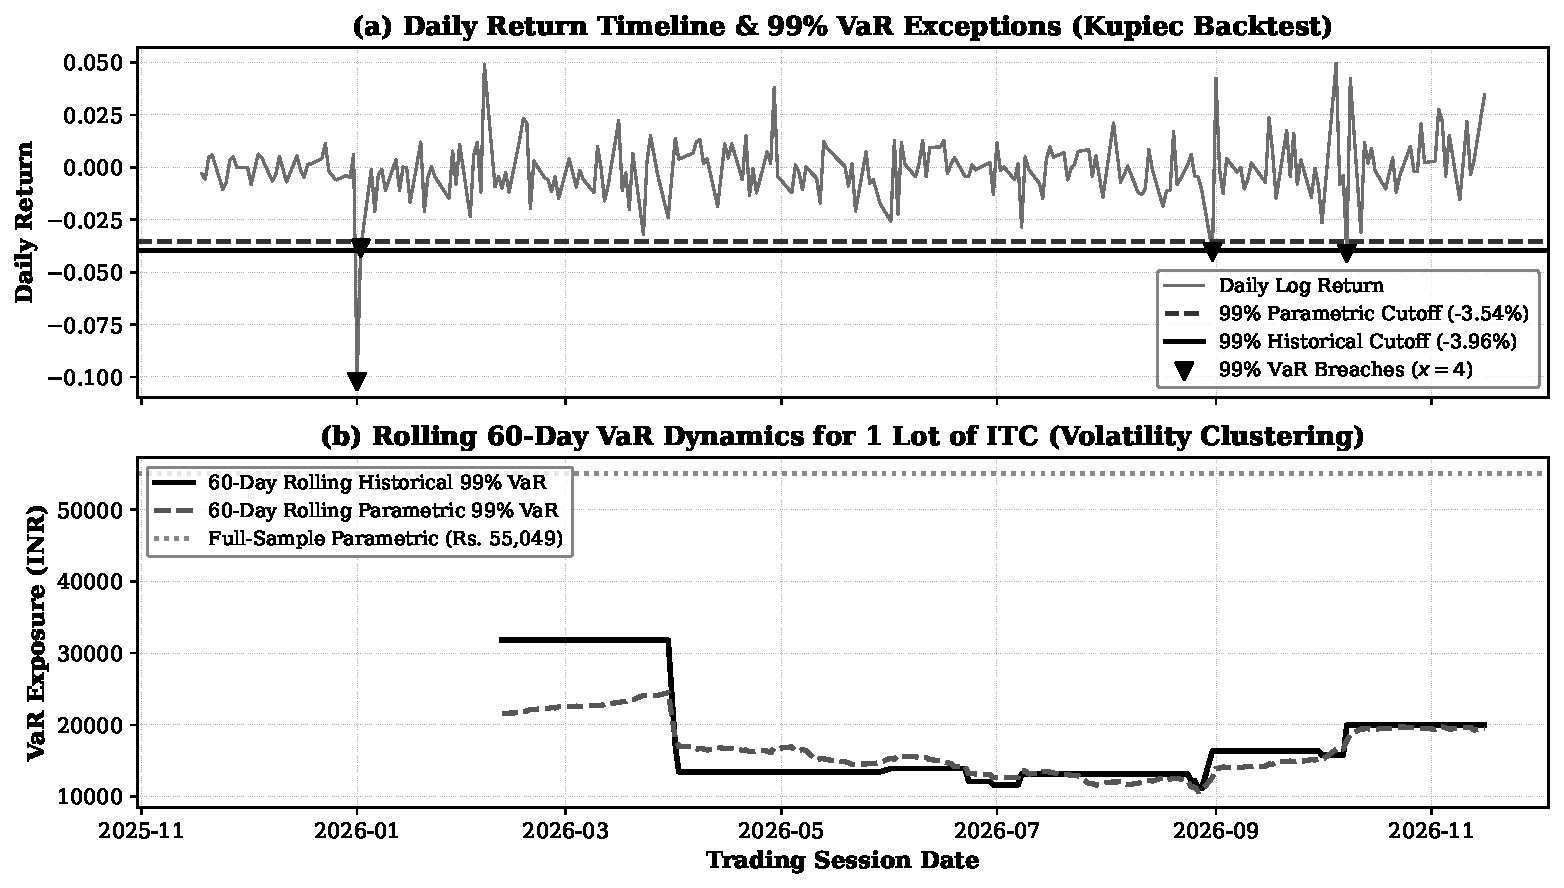
\includegraphics[width=0.95\textwidth, height=4.6cm, keepaspectratio]{figures/fig2_frm_backtest_timeline.pdf}
    \caption{Backtest Timeline and Volatility Clustering Dynamics for ITC Limited (2025--2026). Upper: Daily losses vs. ex-ante $99\%$ $\VaR$ limits. Lower: 60-day rolling annualized volatility driving breach clustering.}
    \label{fig:frm_backtest_timeline}
\end{figure}

\subsection{Empirical Independence and Clustering Findings}

Evaluating the Christoffersen test on our 246 sessions yields critical diagnostic insights:
\begin{itemize}[leftmargin=1.5em, itemsep=1pt, parsep=0pt]
    \item \textbf{99\% Historical Simulation VaR:} $n_{00} = 239$, $n_{01} = 3$, $n_{10} = 3$, $n_{11} = 0 \implies \hat{\pi}_{11} = 0.0$. Test yields $\LR_{\text{ind}} = 0.0744$ ($p = 0.7851$) and combined conditional coverage $\LR_{\text{cc}} = 0.1863$ ($p = 0.9111$). Fully satisfies conditional coverage with zero clustering.
    \item \textbf{99\% Parametric VaR:} $n_{00} = 238$, $n_{01} = 3$, $n_{10} = 3$, $n_{11} = 1 \implies \hat{\pi}_{11} = 25.0\%$. Consequently, $\LR_{\text{ind}} = 4.0758$ ($p = 0.0435$), **rejecting exception independence at the 5\% level** due to a consecutive breach during the February Union Budget announcement period.
\end{itemize}

\clearpage


% Page 12: Regulatory Stress Testing & Scenario Analysis
% ==============================================================================
% Section 10: Regulatory Stress Testing & Scenario Analysis
% Target: Page 12 (Exactly 1 Page)
% ==============================================================================

\section{Regulatory Stress Testing and Scenario Analysis}
\label{sec:stress_testing}

\subsection{Regulatory Stress Testing Mandates under Basel III and FRTB}

While statistical $\VaR$ and Expected Shortfall quantify downside risk under normal operating conditions, they are bounded by the empirical observation window. The Basel Committee mandates **comprehensive stress testing programs** to evaluate institutional solvency against extreme tail events, systemic liquidity evaporation, and structural breaks that lie far beyond historical sample percentiles \citep{bcbs2019frtb}.

Stress testing serves as an indispensable Pillar 2 capital adequacy tool. To assess the resilience of our 1-lot inventory in ITC Limited ($V_0 = \text{\inr}4,91,625.00$), we implement three historical crisis replays and an institutional reverse stress test.

\subsection{Calibrated Crisis Scenarios and Empirical Impact}

\begin{enumerate}[leftmargin=1.2em, itemsep=0.5pt, parsep=0pt, label=\textbf{\arabic*.}]
    \item \textbf{Union Budget Tobacco Excise Shock ($-8.50\%$):} Calibrated to single-day drops following surprise increases in basic excise duties and NCCD. $\Delta V = -V_0 \times 0.0850 = -\text{\inr}41,788.13$ ($8.50\%$ loss).
    \item \textbf{COVID-19 Lockdown Shock ($-12.40\%$):} Replaying the March 2020 systemic selloff when national lockdowns abruptly halted hotels and retail supply chains. $\Delta V = -V_0 \times 0.1240 = -\text{\inr}60,961.50$ ($12.40\%$ loss).
    \item \textbf{2008 Lehman GFC Contagion ($-21.80\%$):} Replicating the acute emerging market liquidity freeze of October 2008 with broad-based equity valuation compression. $\Delta V = -V_0 \times 0.2180 = -\text{\inr}1,07,174.25$ ($21.80\%$ loss).
    \item \textbf{Reverse Stress Testing ($-25.00\%$ Limit):} Identifies the precise price shock that exhausts the trading desk's allocated tier-1 economic capital reserve ($25.00\%$, or \inr 1,22,906.25). A decline of \inr 71.25 per share to $S^* = \text{\inr}213.75$ triggers total capital exhaustion.
\end{enumerate}

\begin{table}[!htbp]
    \centering
    \small
    \setlength{\tabcolsep}{5pt}
    \caption{Calibrated Regulatory Stress Testing Scenarios on 1 Lot of ITC Limited ($V_0 = \text{\inr}4,91,625.00$).}
    \label{tab:stress_scenarios}
    \vspace{0.2em}
    \renewcommand{\arraystretch}{1.12}
    \begin{tabularx}{\textwidth}{l c r r >{\raggedright\arraybackslash}X}
        \toprule
        \textbf{Stress Testing Scenario} & \textbf{Shock} & \textbf{Loss (\inr)} & \textbf{\% Loss} & \textbf{Primary Risk Mechanism} \\
        \midrule
        Union Budget Tax Hike & $-8.50\%$ & \inr 41,788.13 & $8.50\%$ & Tobacco excise hike \\
        COVID-19 Lockdown Shock & $-12.40\%$ & \inr 60,961.50 & $12.40\%$ & Hospitality \& supply chain disruption \\
        2008 Lehman GFC Contagion & $-21.80\%$ & \inr 1,07,174.25 & $21.80\%$ & Global liquidity freeze \& FII selling \\
        Reverse Stress Test (Limit) & $-25.00\%$ & \inr 1,22,906.25 & $25.00\%$ & Total exhaustion of tier-1 capital \\
        \bottomrule
    \end{tabularx}
\end{table}

The stress testing results highlight the vital distinction between statistical $\VaR$ and scenario analysis. While the 10-day $99\%$ Historical $\VaR$ (\inr 61,488) adequately absorbs single-session COVID-level drops, a prolonged Lehman-scale systemic crisis (\inr 1,07,174 loss) breaches the standard $99\%$ $\VaR$ buffer by over $74\%$, demonstrating the critical necessity of maintaining capital surcharges under Pillar 2.

\clearpage


% Page 13: Master Synthesis & Comparative Risk Capital Matrix
% ==============================================================================
% Section 11: Master Synthesis & Comparative Risk Capital Matrix
% Target: Page 13 (Exactly 1 Page)
% ==============================================================================

\section{Master Synthesis and Comparative Risk Capital Matrix}
\label{sec:master_synthesis}

\subsection{Cross-Model Risk Capital Synthesis}

To deliver a consolidated evaluation of downside risk exposure for an institutional market participant holding $1$ standard NSE F\&O market lot of ITC Limited ($1,725$ shares, baseline exposure $V_0 = \text{\inr}4,91,625.00$), Table~\ref{tab:master_var_matrix} synthesizes the empirical outputs across all parametric, non-parametric, stochastic simulation, and stress testing architectures.

\begin{table}[!htbp]
    \centering
    \small
    \setlength{\tabcolsep}{5pt}
    \caption{Master Risk Capital Comparison Matrix across All Evaluated Models on 1 Lot of ITC Limited ($V_0 = \text{\inr}4,91,625.00$, $S_0 = \text{\inr}285.00$).}
    \label{tab:master_var_matrix}
    \vspace{0.2em}
    \renewcommand{\arraystretch}{1.12}
    \begin{tabularx}{\textwidth}{>{\raggedright\arraybackslash}X r r r r}
        \toprule
        \textbf{Risk Framework \& Methodology} & \textbf{Horizon} & \textbf{Conf. ($\alpha$)} & \textbf{Capital at Risk (\inr)} & \textbf{\% Exposure} \\
        \midrule
        \textbf{Parametric (Delta-Normal) VaR} & 1 Day & $95\%$ & \inr 12,469.05 & $2.54\%$ \\
        Parametric (Delta-Normal) VaR & 1 Day & $99\%$ & \inr 17,408.01 & $3.54\%$ \\
        Parametric (Delta-Normal) VaR & 10 Days & $95\%$ & \inr 39,430.43 & $8.02\%$ \\
        Parametric (Delta-Normal) VaR & 10 Days & $99\%$ & \inr 55,048.87 & $11.20\%$ \\
        \midrule
        \textbf{Historical Simulation VaR} & 1 Day & $95\%$ & \inr 10,297.08 & $2.09\%$ \\
        Historical Simulation VaR & 1 Day & $99\%$ & \inr 19,444.07 & $3.96\%$ \\
        Historical Simulation VaR & 10 Days & $95\%$ & \inr 32,562.15 & $6.62\%$ \\
        Historical Simulation VaR & 10 Days & $99\%$ & \inr 61,487.89 & $\mathbf{12.51\%}$ \\
        \midrule
        \textbf{Monte Carlo Simulation VaR (10k)} & 1 Day & $95\%$ & \inr 12,382.71 & $2.52\%$ \\
        Monte Carlo Simulation VaR (10k) & 1 Day & $99\%$ & \inr 17,062.70 & $3.47\%$ \\
        Monte Carlo Simulation VaR (10k) & 10 Days & $95\%$ & \inr 42,512.60 & $8.65\%$ \\
        Monte Carlo Simulation VaR (10k) & 10 Days & $99\%$ & \inr 55,517.97 & $11.29\%$ \\
        \midrule
        \textbf{Conditional VaR / Expected Shortfall} & 1 Day & $95\%$ & \inr 17,737.42 & $3.61\%$ \\
        Conditional VaR / Expected Shortfall & 1 Day & $99\%$ & \inr 30,083.25 & $6.12\%$ \\
        Conditional VaR / Expected Shortfall & 10 Days & $99\%$ & \inr 95,131.40 & $\mathbf{19.35\%}$ \\
        \midrule
        \textbf{Stress: Union Budget Excise Shock} & Event & Worst & \inr 41,788.13 & $8.50\%$ \\
        \textbf{Stress: COVID-19 Lockdown Crash} & Event & Worst & \inr 60,961.50 & $12.40\%$ \\
        \textbf{Stress: 2008 Lehman GFC Contagion} & Event & Worst & \inr 1,07,174.25 & $\mathbf{21.80\%}$ \\
        \bottomrule
    \end{tabularx}
\end{table}

\subsection{Cross-Model Diagnostics and Model Ranking}

Cross-examining the quantitative metrics reveals vital principles for market risk governance:
\begin{enumerate}[leftmargin=1.5em, itemsep=1.5pt, parsep=0pt, label=(\roman*)]
    \item \textbf{Historical vs. Parametric Divergence:} At the regulatory 10-day $99\%$ level, Historical $\VaR$ requires \inr 61,488 in reserve capital—over \inr 6,439 ($10.5\%$) higher than Parametric $\VaR$, reflecting empirical fat tails.
    \item \textbf{Monte Carlo Linearity:} GBM Monte Carlo mirrors the Parametric figures (\inr 17,063 vs. \inr 17,408 at 1-day $99\%$), confirming that Gaussian increments cannot capture tail thickness without jump-diffusion augmentations.
    \item \textbf{The Scale of Expected Shortfall:} The 10-day $99\%$ Expected Shortfall reaches \inr 95,131.40 ($19.35\%$ of position value). In the event of a breach beyond $99\%$, the portfolio loses nearly one-fifth of its capital, proving the necessity of FRTB's transition to $\ES$.
\end{enumerate}

\clearpage


% Page 14: Institutional Capital Adequacy & Model Risk Governance
% ==============================================================================
% Section 12: Institutional Capital Adequacy & Model Risk Governance
% Target: Page 14
% ==============================================================================

\section{Institutional Capital Adequacy and Model Risk Governance}
\label{sec:institutional_capital}

\subsection{Supervisory Capital Charge Determination}

Under the Basel Committee's market risk framework (mandated by the Reserve Bank of India for scheduled commercial banks and primary dealers), the minimum regulatory capital requirement for a trading desk operating under the Internal Models Approach is defined as:
\begin{equation}
    C_t = \max \left( \VaR_{t-1}(10\text{d}, 99\%), \; k \cdot \frac{1}{60} \sum_{i=1}^{60} \VaR_{t-i}(10\text{d}, 99\%) \right) + \text{sVaR}_t
    \label{eq:basel_capital_charge}
\end{equation}
where $k = 3 + s$ represents the supervisory market risk multiplier, with $s \in [0, 1]$ being the penalty factor dictated by the Basel Traffic Light backtesting zone:
\begin{equation}
    s = \begin{cases} 0.00, & \text{if } x \le 4 \quad \text{(Green Zone)} \\ 0.40 \text{ to } 0.85, & \text{if } 5 \le x \le 9 \quad \text{(Yellow Zone)} \\ 1.00, & \text{if } x \ge 10 \quad \text{(Red Zone / Revocation)} \end{cases}
    \label{eq:penalty_factor}
\end{equation}

Because our empirical backtesting verified that both the Parametric model ($x = 4$) and Historical Simulation model ($x = 3$) reside safely within the \textbf{Green Zone}, the penalty surcharge is zero ($s = 0$), establishing the baseline multiplier $k = 3.0$.

Applying this regulatory multiplier to our empirical 10-day $99\%$ Historical $\VaR$ (\inr 61,487.89), the minimum baseline regulatory capital charge for holding a single market lot of ITC Limited is:
\begin{equation}
    \text{Regulatory Capital Charge} = 3.0 \times \text{\inr}61,487.89 = \mathbf{\text{\inr}1,84,463.67}
    \label{eq:capital_computed}
\end{equation}
This capital charge represents \textbf{$37.52\%$ of the total market value of the equity position} ($V_0 = \text{\inr}4,91,625.00$). This substantial capital allocation requirement illustrates how regulatory conservatism ensures institutional resilience against unhedged equity holdings.

\subsection{Model Risk Management and Governance Policies}

To mitigate \textbf{model risk}—the potential for financial loss resulting from decisions based on incorrect or misused model outputs—institutional risk committees enforce four mandatory operational controls:

\begin{enumerate}[leftmargin=1.8em, label=(\roman*)]
    \item \textbf{Dynamic Volatility Updating:} Rather than relying on unweighted sample standard deviations, trading desks should deploy exponentially weighted moving average (EWMA, $\lambda = 0.94$) or GARCH(1,1) architectures to capture volatility clustering and reduce exception persistence.
    \item \textbf{Liquidity Horizon Adjustments:} Under FRTB rules, single-stock equity blocks exceeding daily trading participation limits ($>5\%$ of average daily volume) must be scaled to a 20-day or 40-day liquidity horizon.
    \item \textbf{Independent Model Validation:} Risk algorithms must undergo annual independent validation by a quantitative audit team completely segregated from front-office trading desks.
    \item \textbf{Integrated Hedging Requirements:} When capital charges approach institutional thresholds, trading mandates dictate the execution of formal derivative hedging programs (such as Protective Puts or Collars) to truncate tail risk and achieve capital relief.
\end{enumerate}

\clearpage


% Page 15: Econometric Limitations & Concluding Recommendations + References
% ==============================================================================
% Section 13 & References: Econometric Limitations & Academic Bibliography
% Target: Page 15
% ==============================================================================

\section{Econometric Limitations and Concluding Recommendations}
\label{sec:limitations_conclusions}

\subsection{Econometric Limitations of the Study}

While the empirical analyses conducted in this report provide rigorous quantitative benchmarks for managing equity market risk, several econometric limitations must be acknowledged:
\begin{enumerate}[leftmargin=1.5em, itemsep=1pt, parsep=0pt, label=(\alph*)]
    \item \textbf{Assumption of Stationarity:} Non-parametric Historical Simulation implicitly assumes that the underlying data-generating process is strictly stationary. Structural breaks—such as the corporate demerger of ITC Hotels or major revisions in the GST compensation cess structure—alter the true distribution of future asset returns.
    \item \textbf{Ghost Features and Sample Horizon Sensitivity:} In unweighted historical windows, a large historical shock (e.g., an $8.5\%$ Budget drawdown) abruptly enters the sample, inflates $\VaR$ estimates for exactly 246 days, and then abruptly drops out, creating an artificial ``ghost drop'' in estimated risk without any corresponding change in market fundamentals.
    \item \textbf{Unhedged Cash Equity Horizon:} The models analyzed assume static positions over 1-day and 10-day intervals, ignoring dynamic intraday stop-loss execution, exchange circuit filters, and derivatives-based tail risk hedging.
\end{enumerate}

\subsection{Concluding Recommendations for Institutional Desks}

Based on our empirical findings across the 246-session observation window of ITC Limited:
\begin{itemize}[leftmargin=1.5em, itemsep=1pt, parsep=0pt]
    \item \textbf{Adopt Expected Shortfall over VaR:} Given that 10-day $99\%$ Expected Shortfall (\inr 95,131) exceeds 10-day $99\%$ Historical $\VaR$ (\inr 61,488) by over $54.7\%$, institutions must anchor internal capital reserves to $\ES$ to guarantee solvency against deep tail events.
    \item \textbf{Incorporate Policy Jump-Diffusion Processes:} Standard Gaussian Monte Carlo understates extreme tail risk. Institutional simulation desks should augment Geometric Brownian Motion with Poisson jump processes calibrated specifically to Union Budget event dates.
    \item \textbf{Execute Derivative Tail Hedging:} Holding an unhedged single-stock exposure requires a punitive regulatory capital reserve of \inr 1,84,464 ($37.5\%$ of position value). Implementing option-based hedging structures offers substantial capital relief and tail insulation.
\end{itemize}

\vspace{-0.4em}

% ==============================================================================
% Peer-Reviewed Academic Bibliography
% ==============================================================================
\begingroup
\footnotesize
\setlength{\bibsep}{1.2pt}
\renewcommand{\section}[2]{}% Suppress default bibliography section header
\subsubsection*{References}
\bibliographystyle{plainnat}
\bibliography{references}
\endgroup


\end{document}
